\documentclass{article}
\usepackage[margin=1in]{geometry}
\usepackage{amsmath,amsthm,amssymb}
\usepackage{bbm,enumerate,mathtools}
\usepackage{tikz,pgfplots}
\usepackage{chessboard}
\usepackage[hidelinks]{hyperref}
\usepackage{multicol} % Problem 35
\usepackage{xstring} % Difficulty command
\usetikzlibrary{shapes.geometric}

\newenvironment{question}{\begin{trivlist}\item[\textbf{Question.}]}{\end{trivlist}}
\newenvironment{note}{\begin{trivlist}\item[\textbf{Note.}]}{\end{trivlist}}
\newenvironment{references}{\begin{trivlist}\item[\textbf{References.}]}{\end{trivlist}}
\newenvironment{related}{\begin{trivlist}\item[\textbf{Related.}]\end{trivlist}\begin{enumerate}}{\end{enumerate}}

\newcommand\score[1]{
\pgfmathsetmacro\pgfxa{#1+1}
\tikzstyle{scorestars}=[
  star,
  star points=5,
  star point ratio=2.25,
  draw,
  inner sep=3pt,
  anchor=outer point 5
]
  \begin{tikzpicture}[baseline]
    \draw[opacity=0] (0,-0.5) rectangle (0,0.2); % Workaround for whitespace at the bottom.
    \foreach \i in {1,...,4} {
      \pgfmathparse{(\i<=#1?"yellow":"gray")}
      \edef\starcolor{\pgfmathresult}
      \draw (\i*4.5ex,0) node[name=star\i,scorestars,fill=\starcolor]  {};
    }
  \end{tikzpicture}
}

\newcommand{\difficulty}[1]{%
  \IfEqCase{#1}{%
      {1}{
        
\begin{tikzpicture}[scale=0.7, baseline=0.9mm]%
          \definecolor{slopegreen}{rgb}{0.0, 0.5, 0.0}%
          \fill[slopegreen] (0.5,0.5) circle (0.5);%
        \end{tikzpicture}%
      }%
      {2}{
        
\begin{tikzpicture}[scale=0.7, baseline=0.9mm]%
          \definecolor{slopeblue}{rgb}{0.0, 0.44, 1.00}
          \fill[slopeblue] (0,0) rectangle (1,1);%
        \end{tikzpicture}%
      }%
      {3}{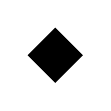
\begin{tikzpicture}[scale=0.7, baseline=0.9mm]\fill (0,0.5)--(0.5, 0)--(1,0.5)--(0.5,1)--cycle; \end{tikzpicture}}%
      {4}{
\begin{tikzpicture}[scale=0.7, baseline=0.9mm]\fill (0.25,0)--(0,0.5)--(0.25,1)--(0.5,0.5)--cycle; \fill (0.75,0)--(0.5,0.5)--(0.75,1)--(1,0.5)--cycle;\end{tikzpicture}}%
      % you can add more cases here as desired
  }[\PackageError{difficulty}{Undefined difficulty level: #1}{}]%
}%
\newcommand{\rating}[2]{\difficulty{#1}\\\score{#2}\\}

\usetikzlibrary{patterns}

\begin{document}
\rating{3}{2}
  Suppose you have two finite groups $G$ and $H$, a $G$-set $X$, and a target
  function $t\colon X\rightarrow H$.
  \\
  You want to construct some finite sequence of maps
  $\{f_i\colon X \rightarrow H\}_{i=1}^N$ such that for any
  function $s_0\colon X \rightarrow H$ and any sequence $\{g_i \in G\}_{i=1}^{N-1}$
  the following sequence contains $t$ \[
    \{
      s_0(x),
      \underbrace{f_1(x) \cdot s_0(x)}_{s_1},
      \underbrace{f_2(x) \cdot g_1 * s_1(x)}_{s_2},
      \hdots,
      \underbrace{f_{N}(x) \cdot g_{N-1} * s_{N-1}(x)}_{s_N}\}
  \] where $f_i(x) \cdot s(x) = f_i(x)s(x)$ under ordinary group multiplication,
  and $g_i * s(x) = s(g_i^{-1}x)$.

\begin{figure}[ht!]
  \centering
  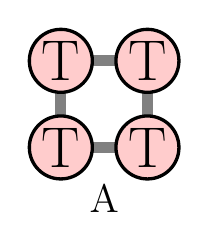
\begin{tikzpicture}
    \draw[gray, line width=4] (0.45,0.45) rectangle (1.55,1.55);
    \draw[very thick, fill=red!20]
      (0.45, 0.45) circle (0.4) node {\huge T}
      (1.55, 0.45) circle (0.4) node {\huge T}
      (0.45, 1.55) circle (0.4) node {\huge T}
      (1.55, 1.55) circle (0.4) node {\huge T};
    \node at (1, -0.2) {\Large A};
  \end{tikzpicture}
  \hspace{0.5cm}
  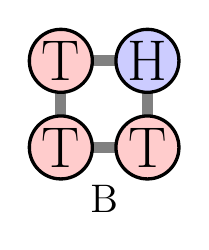
\begin{tikzpicture}
    \draw[gray, line width=4] (0.45,0.45) rectangle (1.55,1.55);
    \draw[very thick, fill=red!20]
      (0.45, 0.45) circle (0.4) node {\huge T}
      (1.55, 0.45) circle (0.4) node {\huge T}
      (0.45, 1.55) circle (0.4) node {\huge T};
    \draw[very thick, fill=blue!20]
      (1.55, 1.55) circle (0.4) node {\huge H};

    \node at (1, -0.2) {\Large B};
  \end{tikzpicture}
  \hspace{0.5cm}
  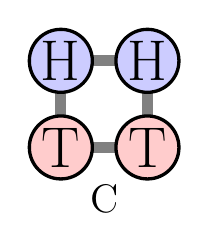
\begin{tikzpicture}
    \draw[gray, line width=4] (0.45,0.45) rectangle (1.55,1.55);
    \draw[very thick, fill=red!20]
      (0.45, 0.45) circle (0.4) node {\huge T}
      (1.55, 0.45) circle (0.4) node {\huge T};
    \draw[very thick, fill=blue!20]
      (0.45, 1.55) circle (0.4) node {\huge H}
      (1.55, 1.55) circle (0.4) node {\huge H};

    \node at (1, -0.2) {\Large C};
  \end{tikzpicture}
  \hspace{0.5cm}
  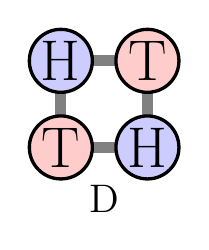
\begin{tikzpicture}
    \draw[gray, line width=4] (0.45,0.45) rectangle (1.55,1.55);
    \draw[very thick, fill=red!20]
      (0.45, 0.45) circle (0.4) node {\huge T}
      (1.55, 1.55) circle (0.4) node {\huge T};
    \draw[very thick, fill=blue!20]
      (1.55, 0.45) circle (0.4) node {\huge H}
      (0.45, 1.55) circle (0.4) node {\huge H};

    \node at (1, -0.2) {\Large D};
  \end{tikzpicture}
  \\
  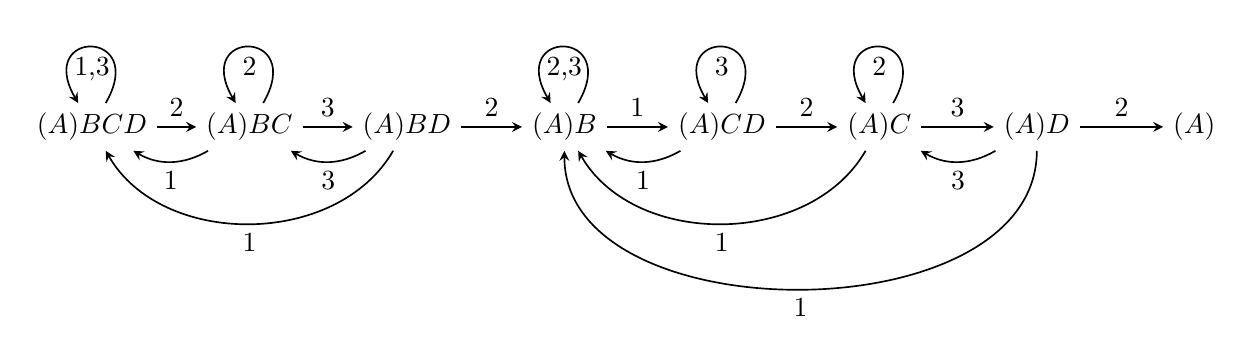
\begin{tikzpicture}[
    > = stealth, % arrow head style
    auto,
    node distance = 2cm, % distance between nodes
    semithick % line style
  ]
    \node (a) {$(A)BCD$};
    \node (b) [right of=a] {$(A)BC$};
    \node (c) [right of=b] {$(A)BD$};
    \node (d) [right of=c] {$(A)B$};
    \node (e) [right of=d] {$(A)CD$};
    \node (f) [right of=e] {$(A)C$};
    \node (g) [right of=f] {$(A)D$};
    \node (h) [right of=g] {$(A)$};

    \draw[looseness=8,out=60,in=120,->] (a) edge node {1,3} (a);
    \draw[->] (a) edge node {2} (b);
    \draw[->] (b) edge node {3} (c);
    \draw[->] (c) edge node {2} (d);
    \draw[->] (d) edge node {1} (e);
    \draw[->] (e) edge node {2} (f);
    \draw[->] (f) edge node {3} (g);
    \draw[->] (g) edge node {2} (h);

    \draw[looseness=8,out=60,in=120,->] (b) edge node {2} (b);
    \draw[looseness=1,out=210,in=330,->] (b) edge node {1} (a);

    \draw[looseness=1,out=240,in=300,->] (c) edge node {1} (a);
    \draw[looseness=1,out=210,in=330,->] (c) edge node {3} (b);

    \draw[looseness=8,out=60,in=120,->] (d) edge node {2,3} (d);

    \draw[looseness=1,out=210,in=330,->] (e) edge node {1} (d);
    \draw[looseness=8,out=60,in=120,->] (e) edge node {3} (e);

    \draw[looseness=8,out=60,in=120,->] (f) edge node {2} (f);
    \draw[looseness=1,out=240,in=300,->] (f) edge node {1} (d);

    \draw[looseness=1,out=210,in=330,->] (g) edge node {3} (f);
    \draw[looseness=1,out=270,in=270,->] (g) edge node {1} (d);
  \end{tikzpicture}
  \caption{
    Let $X$ be the vertices of the square $G = C_4$ the cyclic group which acts
    on the $X$ by rotation, $H = \mathbb Z_2$, and $t(x) \equiv 0$.
    Then interspersing the above sequence of $N=7$ moves with $f(x) = 1$ will
    always result in the sequence reaching the target function, where $1, 2,$
    and $3$ are the moves that flip one coin, two opposite coins, and
    two adjacent coins respectively.
  }
\end{figure}
\begin{question}
  What conditions on $G, H, X$ and $t$ guarantee such a finite sequence of maps?
\end{question}

\begin{related}
  \item Given $G, H, X$ and $t$, what is the minimum $N$?
  \item If the sequence $\{g_i \in G\}_{i=1}^\infty$ is chosen uniformly at
  random, what is the expected length of $\{f_i\}$ before $t$ is reached?
  \item What if there is a set of target functions, any one of which is valid.
  (e.g. all sets satisfying the condition that the number of heads is congruent
  to $2 \pmod 3$.)
  \item Can this be generalized to multiple dimensions (e.g. a tetrahedron)?
  \item What if something about $s_i$ is told to you after the $i$th move for each
    $i$ (and the strategy can depend on this information)?
\end{related}

\begin{note}
  This can be generalized to an arbitrary $2^n$-gon, but no other $m$-gon.
  The idea is that (1) you can't solve any $m$-gon with $m$ odd, and (2) you
  can solve a $m$-gon if and only if you can solve a $d$-gon for every proper
  divisor $d \mid m$.
\end{note}

\begin{references}
  \item \url{http://mathriddles.williams.edu/?p=77}
\end{references}
\end{document}
